%# -*- coding: utf-8-unix -*-
%%==================================================
%% chapter_1.tex for SJTU Master Thesis
%%==================================================

\chapter{概述}
\label{chap:intro}
随着当前网络通信与计算机技术的不断发展,在工业领域中越来越多的基于网络的分布式系统的到了嘤嘤。而随着这些系统的物理范围不断扩大,也为了保证分布式网络系统能够实现精确的数据采集、运行控制等实时性任务,工业中对于各个分布式节点的时间同步精度提出了极为严格的要求,尤其是在大多数以工业以太网为基础的控制系统中,已经逐渐对同步精度提出了微秒级甚至纳秒级别的要求。但是,由于实际测控设备之间固有的时钟差异和时钟数据在网络传输中的随机延时,而且现场设备会由于温度变化、电磁干扰、振荡器老化等多种原因而使得自身时钟并不稳定,使得时间误差随时间不断累积,严重破坏了如变电站、电力监控系统等对时钟同步严格的工业应用。因此,必须追求一种更加有效且高精度的时钟同步技术来提高系统内部节点之间的时钟同步精度。

\section{时钟同步在工业领域的发展历程}
\subsection{时钟同步概念}
\label{sec:concept}
时钟同步即保证工业系统内各个节点的时钟能够保持一致,即维护一个全局一致的物理或逻辑时钟,使得系统各节点中与时间有关的信息、时间及行为有一个全局一致的解释\supercite{1}。
常说的时钟同步,主要包含了时刻同步和时间间隔一致。时刻即表示连续流逝时间的某一个瞬间,而时间间隔是指两个时刻之间的间隔长度。所以,时钟同步主要包括频率同步和相位同步两个方面:
\begin{itemize}[noitemsep,topsep=0pt,parsep=0pt,partopsep=0pt]
	\item 频率同步(Frequency Synchronization):
		所谓频率同步是指各从时钟自身运行的计数器频率保持相同平均速率。通过频率同步可以保持所有节点以相同的计数频率运行,从而极大减小时钟误差根源,降低了累积时钟误差。频率同步必须依靠接受连续的时钟信息才能计算出真实的频率并对自身作出调整。
	\item 相位同步(Phase Synchronization):
		相位便是对频率的积分。通过将时钟的相位量化,赋予数值表示,就是时刻。相位同步可以接受离散的时间信息来调整本地时钟。
\end{itemize}

所以说,时钟同步主要是完成对时和守时这两个功能,所谓“对时”,就是通过不定期的对表操作,来将本地时钟的相位与远程节点相位进行同步;守时就是保持频率一致,尽可能的让本地节点和远程节点的时间间隔偏差在一个允许的范围内。

\subsection{现有时钟同步技术分析}
\label{sec:sync_methods}
在工业领域时钟同步技术不断发展,人们研究使用了如GPS、包时钟同步技术等主流方案来进行时钟同步。下面作简单介绍。
\subsubsection{GPS同步技术}
如超高压变电站等工业系统对于时间同步精度的要求非常高,例如变电站运行人员实时监控电网运行,一旦发生事故后的故障分析,这些都需要统一的时间基准。而以全球定位系统GPS作为时间基准,可以提供非常高的同步精度(达到50ns),而且这种方式不依赖通络的数据负载,直接传递频率和相位信息,让整个系统保持极高的同步性能。

然而,这种方式也存在自身弊端。
\begin{itemize}[noitemsep,topsep=0pt,parsep=0pt,partopsep=0pt]
	\item GPS不适用于室内节点,存在难以选址和安装的问题,这使得GPS同步技术的人力成本增大。
	\item GPS设备本身价格昂贵,而且人们一般会选取高昂的晶振用作备用时钟,以保持系统的安全性。而且若GPS设备大量使用,可想而知后期的更换升级的费用也会十分高昂。
	\item 由于美国政府从未对GPS信号的质量及使用期限给予任何承若何保证,而且美国政府还具有对特定地区GPS信号严重降质处理的能力,所以大量使用GPS会存在严峻的国防安全隐患。
\end{itemize}

\subsubsection{包时钟同步技术}
所谓包时钟同步技术ToP\footnote{Timing over Packet},就是利用分组网络来传递时间信息,而所传递的时间报文也有多种。
\begin{itemize}[noitemsep,topsep=0pt,parsep=0pt,partopsep=0pt]
	\item  NTP(Network Time Protocol)\footnote{http://www.ntp.org/}协议全称是网络时间协议,主要用来使互联网上计算机保持时间同步,一般而言,NTP可以提供1-50ms的可靠时间源。另外,SNTP(Simple Network Time Protocol)\footnote{http://www.networksorcery.com/enp/protocol/sntp.htm}简单网络时钟同步协议也是较为主流的时间同步协议,它能提供接近1ms的同步精度。然后这两种协议比较容易受到网络突发报文的影响而使得同步精度降低。
	\item PTP(Precise Time Protocol)\footnote{https://en.wikipedia.org/wiki/Precision\_Time\_Protocol}精确时间同步协议,来自于IEEE1588协议标准。该协议第一版于2002年推出,具备亚微秒级的同步精度,允许同时传递频率和相位信息。第二版于2008年公布,缩短并同意了报文长度,并且引入了透明时钟机制。具备更高的时间同步精度。
\end{itemize}

结合对当前所有同步技术的综合分析可以看出,由于GPS严重的国防安全隐患和高昂的使用成本使得我们难以大规模应用这种同步技术,而NTP协议主要应用于互联网中保持计算机时间同步,其精度只能达到毫秒级别,同样不适用于对同步精度要求非常高的工业系统中。而PTP同步技术从实现的简单性、精度要求和稳定性方面都能够很好的满足现如今分布式系统对时间同步精度的要求,因此,本文也选取PTP为主要研究对象。


\section{IEEE1588时钟同步协议}

\subsection{协议介绍}
\label{sec:1588_intro}
IEEE1588标准,即“网络测量和控制系统的精确时钟同步协议”,Precision Clock Synchronization Protocol for Networked Measurement and Control Systems,也称作PTP协议。

自1995年以太网中数据传输速度从10Mb/s提高到100Mb/s后,计算机网络领域一致在尝试解决网络设备时钟同步问题,随后开发出了一套同步协议--网络时间协议NTP \footnote{Network Time Protocol}--来提高网络设备的同步性能。虽然在不断发展中,NTP协议同步精确度不断提高达到200$\mu$s,但是,面对同步精度要求越来越高的网络实时通信、测量仪器与工业控制领域,NTP难以达到它们的要求。

随后,网络精密时钟同步委员会于2002年在IEEE标准委员会的支持下,推出了IEEE1588时钟同步标准。该标准推出后迅速在Ethernet/IP等基于以太网的总线中得到采用,称为普遍支持的网络对时技术。该协议采用了主从时钟方案,利用报文传递时间信息,基于网络链路的对称性和延时测量技术,来实现主从时钟的频率、相位精确同步。

在2008年,该委员会继续发布了IEEE1588第二版。在第二版标准中,实现了亚微秒级的时钟同步,可以用于军事和实际的测试测量中。而且提供了更为灵活的同步周期、改进了时间戳的表示方法、解决了主时钟容错性能差的问题、提高了网络拓扑变化的适应性。另外,该版本中还引入了透明时钟,增加了端延时机制,有助于明显提高同步精度。

\subsection{PTP协议特点}
\label{sec:1588_features}
PTP协议主要针对分布式网络系统中的精确时钟同步问题,它能够将系统内部各个独立时钟同步到一个统一的时钟标准上,而且消耗的网络和本地资源非常有限,并带来较高的时钟同步精度。如果硬件时钟能够提供硬件级别的时间戳标记功能,那么其同步精度能够达到亚微秒级别。而且PTP协议实现起来成本很低,也非常方便后期的维护工作。

PTP协议与其他时钟同步协议如NTP/SNTP相比,具备如下几个特点:
\begin{itemize}[noitemsep,topsep=0pt,parsep=0pt,partopsep=0pt]
	\item PTP协议适用于局域网中支持组播报文发送的网络通信技术,这种特性决定了该协议非常适合在以太网中实现,不需要经过大的改动就可以在高精度的网络控制系统中运行。
	\item 可以实现亚微秒级别的同步精度,相比之下,NTP/SNTP最多只能达到毫秒级别。
	\item PTP协议所需要的网络资源和计算资源非常少,所以在实现起来消耗的成本不高。
\end{itemize}


\subsection{IEEE1588协议在当前工业领域的应用}
\label{sec:application}
随着IEEE1588协议的不断发展与实践,不仅在测试与测量控制、工业自动化领域广泛应用了该协议,而且随后的军事应用、分组通信和电力系统等多个领域也开始逐步将该同步方法应用进去。在国外,2015年3月在TI推出的高性能多核架构KeyStone\footnote{\url{http://www.eefocus.com/communication/m/339581}}中,提供了两个硬件功能\footnote{KeyStone1支持two step的时间戳模式,同时也能支持1588协议中规定的PTP报文解析}来支持IEEE1588:记录时间戳,发送同步脉冲。在国内,2014年12月,OPWILL\footnote{北京奥普维尔科技有限公司}发布了基于PTN协议分析仪的IEEE1588v2PTP和SyncE测试选件,为运营商提供关键的网络定时和频率同步测试服务来分析全新的IEEE1588v2 PTP和同步以太网(SyncE)协议,从而为运营商的移动回传和LTE测试提供超高性价比测试解决方案\footnote{\url{http://www.c114.net/news/50/a874237.html}}。

\section{IEEE1588实际应用中的主要问题及研究现状分析}
根据IEEE1588协议内容,系统时钟同步精度应该能够达到亚微秒级别\supercite{2}。然而,在实际的应用中,即使严格按照协议标准的内容来实现,仍然难以达到这样的同步精度。例如Padova大学曾严格按照协议标准,实现了一套完整的IEEE1588同步系统\supercite{3},但是在运行中发现同步精度最高只有100微秒,和预期的同步精度还有很大的差距,更何况在工业现场中,更加复杂的工业环境使得同步精度更加难以保证。

\subsection{主要问题}
\label{sec:1588_problem}
首先,我们知道1588协议的同步原理是采用了主从时钟通过时间戳报文来传递时间信息,并通过估计链路延时来计算最终的时间误差并予以校正。然后,我们对1588协议的深入分析及对现场应用情况的深入了解,可以发现以下因素严重破坏了1588实际运行的同步精度。

\subsubsection{时间戳准确度}
\label{sec:1588_problem_timestamp_accu}
首先,1588协议的核心就是通过主从时钟对外发布包含时钟信息的报文来实现所有从时钟向主时钟同步。例如在同步过程中,主时钟会对外发送sync报文,该报文中标记的时间戳在理想情况下应该是报文离开主时钟的一瞬间的时间,但是在实际运行中,由于很多时间戳是在物理层之上标记的,报文被标记时间戳后仍会在协议栈中有短暂滞留,这样导致了发送时间戳的不准确,最终破坏了从时钟的同步计算精度。

\subsubsection{链路不对称性}
\label{sec:1588_problem_route_time_delay}
通过分析1588协议可以看出,从时钟在计算主从时钟偏差时会假设报文传输的往返路径对称,即Master To Slave Delay 和 Slave To Master Delay相等,并据此来求得最终的offset值。严格来讲,这种假设并不成立。首先由于网络传输过程要经过中间节点如交换机等设备,报文在进入这些设备的协议栈会发生排队和堵塞的情况,而这些情况所导致的链路延时变动是无法预知的;另外,报文传输的拓扑结构也并非一成不变的,一旦拓扑结构发生变化,就意味着往返路径可能有极大的不同。这些都是实际运行中链路固有的不对称性表现,所以,如果只是简单按照1588协议中假设路径对称,那么势必会带来不可忽视的误差。

其中,通过我们对实际链路时延的观测,可以发现真实环境中的同步系统中会出现以下几种复杂的数据变动,这些变动会直接破坏从时钟的稳定性和同步精度:
\begin{figure}[!hbp]
  \centering
  \begin{minipage}[b]{0.6\textwidth}
    \captionstyle{\centering}
    \centering
    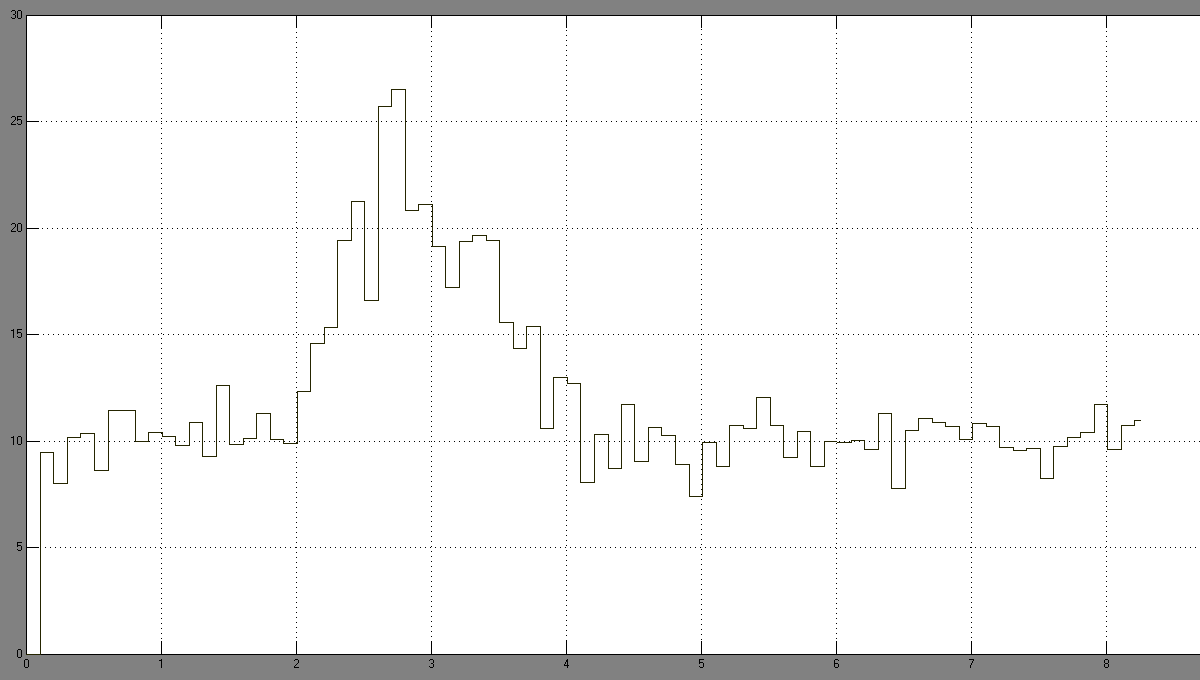
\includegraphics[width=10cm]{matlab/时延暂时性突变曲线}
    \bicaption[fig:curvewithtemporarychange]{时延暂时性突变曲线}{时延暂时性突变曲线}{Fig}{The Curve of time-delay with temporary change}
  \end{minipage}     
\end{figure}

\begin{figure}[!hbp]
  \centering
  \begin{minipage}[b]{0.6\textwidth}
    \captionstyle{\centering}
    \centering
    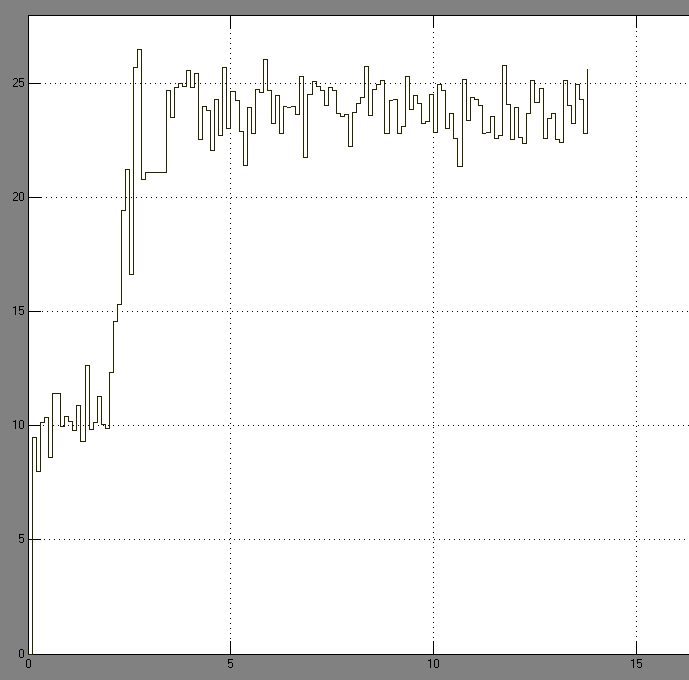
\includegraphics[width=10cm]{matlab/时延持久性变化曲线}
    \bicaption[fig:curvewithpersistentchange]{时延持久性变化曲线}{时延持久性变化曲线}{Fig}{The Curve of time-delay with persistent change}
  \end{minipage}     
\end{figure}

上面的两种时延变化目前在工业中并没有很好的解决方案,所以同步系统会容易受到这两种变化的影响而导致同步精度及稳定性降低。

\subsubsection{网络延时固有抖动}
\label{sec:1588_problem_route_time_delay}
由于1588协议中的报文需要在网络环境下进行传输,而在复杂的网络环境下,报文传输的时间一定会带有随机的抖动漂移,也就是说,即使网络负载良好,拓扑结构也不发生变动的情况下,网络延时仍然会有自身的随机抖动。如果对于这些抖动不进行处理,那么就会导致从时钟不断处于波动之中,甚至有可能导致从时钟系统不稳定。

\subsubsection{从时钟校正策略}
\label{sec:1588_problem_slave_clock_control}
常规的对从时钟校正策略有直接校正和pi控制器校正,其中,直接校正能够快速对从时钟校正,在最短时间内实现时钟同步,然后,一旦offset值计算中存在较大偏差,那么从时钟将处于不断的快速波动当中,这会严重破坏从时钟的同步性能,甚至可能导致从时钟无法稳定。pi控制器是一种较为典型而简单的控制方法,能够保证从时钟较为处于较为稳定的状态,但是,简单的pi控制器并不能考虑到延时的波动对从时钟带来的影响,所以也无法达到很好的控制效果。

\subsection{当今研究现状及其不足}
\label{sec:1588_problem_research}
当前,已经有很多专家学者在对1588协议进行深入研究。针对上述所提出的问题,也有一定的研究成果。
\begin{itemize}[noitemsep,topsep=0pt,parsep=0pt,partopsep=0pt]
	\item 时间戳准确度:为了提高时间戳准确度,尽量使得报文中的时间戳直接来自物理层以可以减少报文在协议栈的停留,2007年推出了首个可以在以太网收发器上集成IEEE1588协议的芯片-DP83640\supercite{4},该芯片能够将时间戳标记点葱原来的应用层下移到数据链路层和物理层之间,从而降低网络流量及协议栈对报文传输延时的影响。又比如,2015年3月TI推出的Keystone架构也同样能够支持物理时间戳标记\supercite{5}。
	\item 链路不对称性:针对链路延时中的不对称性问题,李学桥层提出对主从路径延时和从主路径延时进行加权求平均的方法,其中权值来自于同步报文与延时请求报文的周期比\supercite{6}。在李帅等学者的文献\parencite{7}中提出了一个扩展时钟同步方法来计算不对称路径下的时间偏差。另外,当前主要的解决方法有通过类似透明时钟来记录报文在中间节点的传输时间,并在从时钟处减去传输时间来计算主从偏差。但这种方式在2008年才提出,目前并未得到广泛应用,它不仅会受时间戳精度影响,而且现有大多数同步系统仍然采用的是早期的边界时钟。所以当前并不具备很好的应用价值。在C. Lei的文字\supercite{57}中采用了自适应滤波算法,该算法能较好的进行滤波,但由于不能对历史纪录进行实时分析,从而无法检测持久性的时延变化。
	\item 网络延时固有抖动:Jayesh Chhapekar在2012年发表的一篇文章中对IEEE1588数据包的包延时抖动进行数学分析和建模,并以此来观察数据包延时的概率是如何变化的\supercite{8}。但是在真实的工业环境中,由于网络的复杂性和时变性,我们很难用某个概率分布来拟合固有抖动,所以也很难取得良好的消除抖动效果。文献\parencite{9}中设计了运用卡尔曼滤波算法来计算主从时钟偏差同样有助于减少固有抖动带来的影响。
	\item 从时钟校正策略:当前普遍方法是采用PI控制器进行校正,如文献\parencite{10}中对PI控制器参数选择进行了评估,但是没有详细研究具体的应用方法。另外由于网络的时变性,我们很难用固定的参数来控制从时钟,那样会带来很差的自适应性和鲁棒性。除此之外,文献\parencite{11}对PID控制器在时钟同步中的应用进行深入研究,并且采用了经验法来对PID参数进行整定,但该文缺陷是没有把系统参数发生变化情况下的参数调整考虑进去。文献\parencite{12}利用模糊控制算法来估算时钟偏差,这种方法适合于时钟同步周期较大时,但是如果同步周期太大,网络的不确定性干扰加剧,使得模糊控制的效果变差。
\end{itemize}

\section{本文研究目的及意义}
结合上文可以知道,越来越多的工业领域对时钟同步精度提出了非常高的要求,而传统的NTP和GPS由于使用成本高昂或者同步精度不够而无法满足对应的需求。相较而言,IEEE1588精确时钟同步协议由于其易用性、成本低、精度高等多种优秀特性已经广泛应用于多种工业时钟同步场合,而且随着IEEE1588-2008的推出,其理想精度甚至可以达到亚微秒级,这预示着IEEE1588协议有着极高的研究价值。

另外,在IEEE1588协议的实际应用过程中,我们也通过深入研究分析发现了协议本身存在的多种问题,例如未处理网络延时的不对称性及固有抖动,加之工业网络环境复杂,这使得IEEE1588协议在实际应用中无法达到非常理想的同步精度。而本文便是着手于影响同步精度的因素并通过深入分析来提出本人的解决方案。

具体来说,本文主要立足于以下两点进行深入探讨:
\begin{itemize}[noitemsep,topsep=0pt,parsep=0pt,partopsep=0pt]
	\item 网络传输时延的随机性和不确定性:
在硬件提供高精度时间戳的情况下,网络传输延时误差成为了影响同步精度的最主要来源。因此,本文也着重考察对网络延时问题的解决方法。在文中,本人将网络时延拆分成固有抖动漂移、“暂时性”时延突变和“持久性”时延变化,分别分析各种变化原因,并且从数学统计方法的角度出发,对固有抖动漂移提出基于“线性回归模型”的“时延估计”方法,把历史时延数据作为样本序列,通过回归建模来进行时延估计,从而减小时延抖动或突变对同步精度带来的不良影响;对“暂时性”时延阶跃突变,提出“动态阈值”算法,通过限制阶跃噪声的大小来防止从时钟系统出现过大的振荡;对“持久性”时延变化,提出“基于固定滑动时间窗实时监控”的方法来及早发现持久性变化,并立即通过“样本失效”手段来快速消除持久性变化对“样本序列”及“时延估计”所带来的波动。基于以上本人所提出的算法来保证时延的稳定性、准确性和可靠性。
	\item 从时钟校正的控制策略:
针对从时钟校正策略,本文首先会分析两种应用较为普遍的控制策略:直接校正;pi控制器校正。深入分析这两种策略的优劣。同时,在本人上文中所提出的数学统计方法中,我们会得到足够多的时延样本,利用这些样本数据,本人会提出第三种从时钟控制策略:“基于BP神经网络的PID控制器校正策略”。这种策略可以利用我们前面累计的“原始延时样本”来对神经网络进行训练,而神经网络的输出便是PID三个控制参数。这种策略的好处是能够应对工业网络环境中的复杂性和时变性,通过将统计样本和神经网络相结合,能够使从时钟具备非常好的稳定性和鲁棒性。
\end{itemize}

在文章后面,本人在深入研究所提出的多种“时延统计优化算法”和“基于BP神经网络的PID控制算法”的前提下,通过在自己搭建的基于stateflow的matlab仿真平台上,分别测试了上述所提两种算法。根据最终试验结果表现来观察所提算法对时钟同步系统的稳定性、鲁棒性和自适应性等当面的优化。

\section{论文安排}
以下是本论文的结构安排。

第一章阐述课题背景,需要解决的问题,并且介绍本文主要研究的内容。

第二章介绍1588同步协议的运行原理,同时在最后介绍1588协议在实际运行中遇到的一些不可避免的问题,及对于这些问题的已有研究成果。

第三章从网络传输延时的角度来进行分析,并且提出结合数学统计与实时监控相结合的方法来保证延时数据的稳定性、准确性和可靠性。在该章节会首先对传输延时进行数学模型的建立,通过深入分析其特性可得到数学模型,然后依据模型特性,基于相关的数学统计方法,例如线性回归、固定时间窗等,提出符合模型特性的数学统计优化算法。其中,本人还会提出一套完整的滑动时间窗延时实时监控方案,用以区分“暂时性”延时和“持久性”延时,并在此基础上提出不同的处理方案。从而保证从时钟的稳定性。

第四章从从时钟校正的角度来进行深入研究,首先分析直接校正、pi控制器校正两种方法的原理及优缺点,同时根据这些优缺点,本人提出了基于BP神经网络的智能控制算法来进行PID控制。首先会介绍BP神经网络概念及其原理、应用场景,然后会提出具体的数学方法来在从时钟校正上实现一套较为完整的基于BP神经网络的控制算法,通过原始延时样本对神经网络进行训练,最后通过该算法得出的PID参数进行调节。同时会利用自主搭建的IEEE1588仿真平台上进行实验验证,并对这三种控制方法的控制效果进行比较。从而得出较为完善的控制方法来校正从时钟。另外,在本章中还结合本人实验室所参与的具体工程项目,对时钟同步系统及IEEE1588同步协议的硬件实现做简单的介绍。

第五章会利用我们自己搭建的时钟同步系统仿真平台,并在该平台上对本文中所提到的统计优化算法和基于神经网络PID控制算法进行验证。根据仿真结果得出结论,并总结其中的不足之处。

第六章对全文进行总结和展望。

